\begin{figure}
  \begin{subfigure}{.5\textwidth}
    \centering
    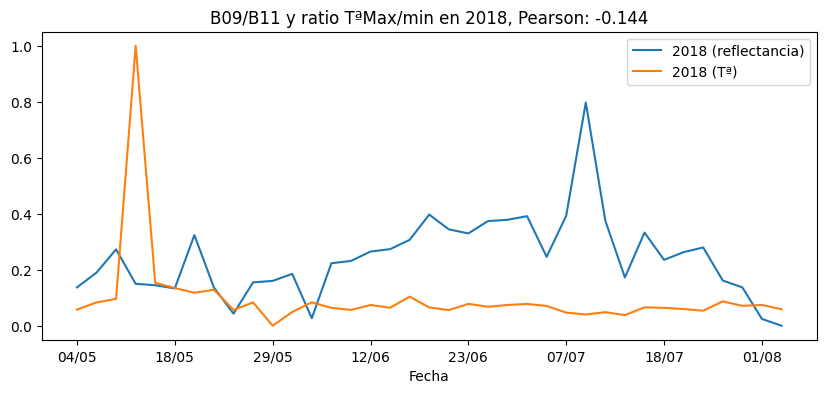
\includegraphics[width=1\linewidth]{figures/separadas_ratioTas+combs/0.png}
    \caption{}
  \end{subfigure}
  \begin{subfigure}{.5\textwidth}
    \centering
    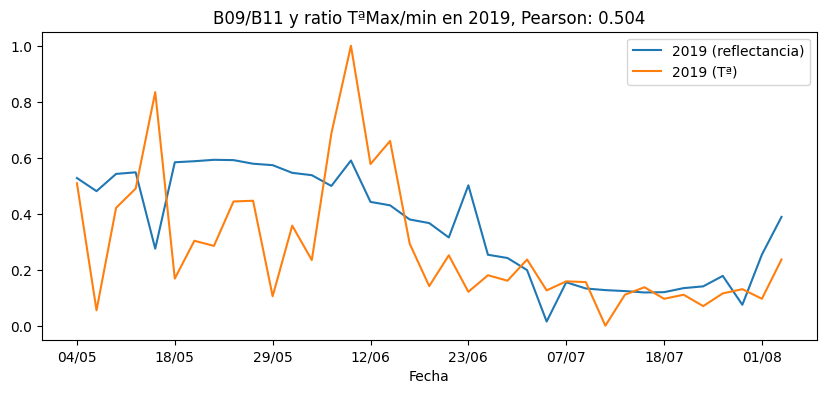
\includegraphics[width=1\linewidth]{figures/separadas_ratioTas+combs/1.png}
    \caption{}
  \end{subfigure}
  \begin{subfigure}{.5\textwidth}
    \centering
    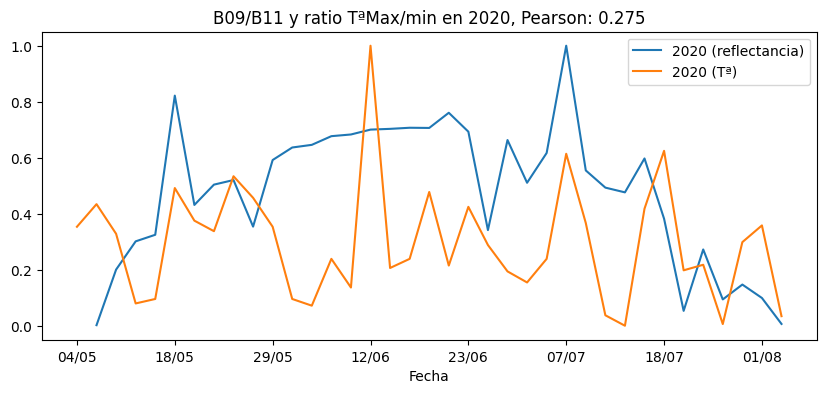
\includegraphics[width=1\linewidth]{figures/separadas_ratioTas+combs/2.png}
    \caption{}
  \end{subfigure}
  \begin{subfigure}{.5\textwidth}
    \centering
    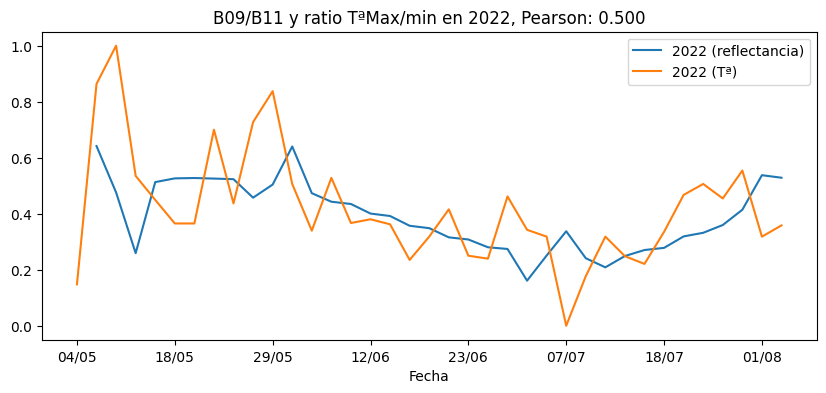
\includegraphics[width=1\linewidth]{figures/separadas_ratioTas+combs/3.png}
    \caption{}
  \end{subfigure}
  \begin{subfigure}{.5\textwidth}
    \centering
    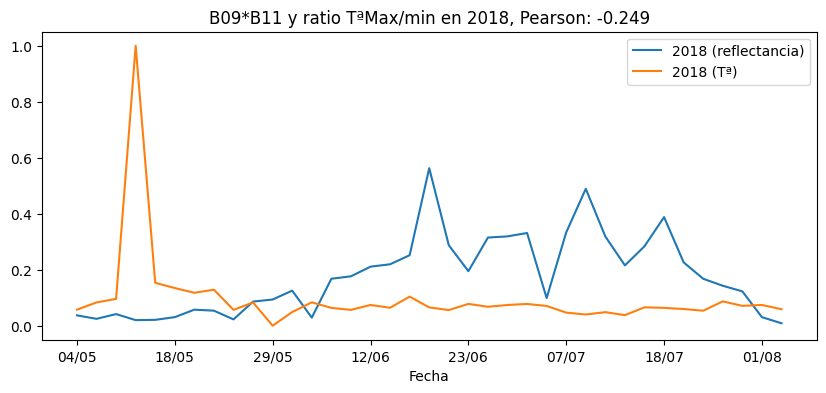
\includegraphics[width=1\linewidth]{figures/separadas_ratioTas+combs/4.png}
    \caption{}
  \end{subfigure}
  \begin{subfigure}{.5\textwidth}
    \centering
    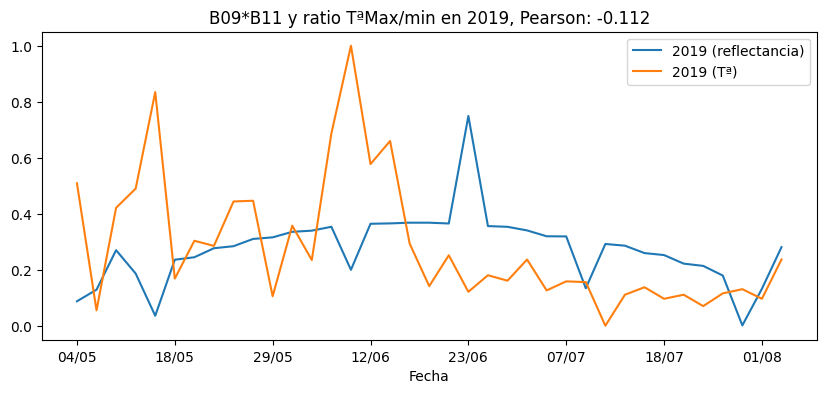
\includegraphics[width=1\linewidth]{figures/separadas_ratioTas+combs/5.png}
    \caption{}
  \end{subfigure}
  \begin{subfigure}{.5\textwidth}
    \centering
    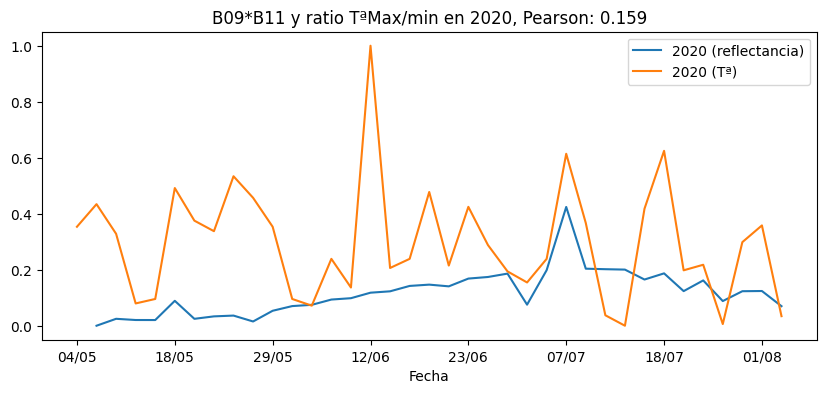
\includegraphics[width=1\linewidth]{figures/separadas_ratioTas+combs/6.png}
    \caption{}
  \end{subfigure}
  \begin{subfigure}{.5\textwidth}
    \centering
    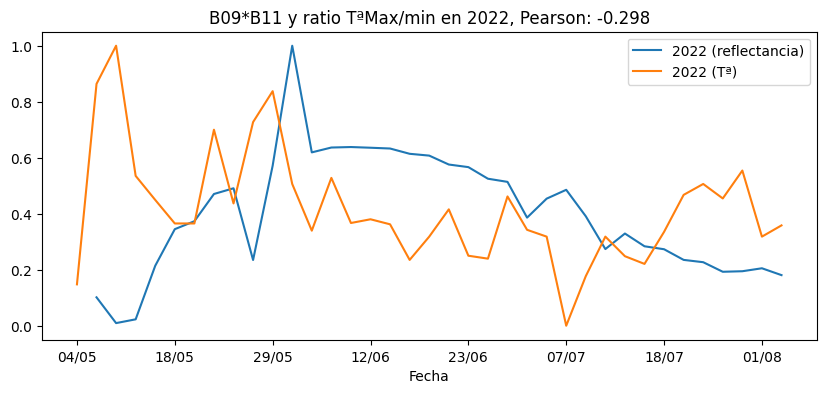
\includegraphics[width=1\linewidth]{figures/separadas_ratioTas+combs/7.png}
    \caption{}
  \end{subfigure}
    \caption{Curvas del ratio TªMax/min y de las combinaciones estudiadas año por año}
    \label{fig:separadas_ratioTas+combs}
\end{figure}